\subsection{\cgrid{} Topology}
\cgrid{} topologies refer geo-referenced locations and
geometries that can be defined analytically, e.g., rectilinear or
curvilinear grids. Storing \cgrid{} topologies amount to storing the
closed form formula. Algorithms for processing \cgrid{}s such as
finding nearest neighbors or finding points that fall withing a
polygonal subset are computed directly using the implicit \cgrid{}
representation, incurring computational overhead.

\subsection{\ugrid{} Topolgy}
A \ugrid{} topology is  defined as a topology that is not regular, i.e.,
do not admit a closed form representation. \ugrid{} topologies offer
the highest level of flexibility from a visualization and modeling
standpoint as a higher sampling frequency may be used regions of
interest and less samples allocated for low-impact areas. 

Any NCML file which exposes the topology of an externally hosted
dataset according to the \cfugrid{} sepcification can be processed by
\sciwms{}. According the \cfugrid{} standard, a topology is always
embedded on the real line, in the real plane or in space with the
locations of a \ugrid{} topology's vertices exposed as an array of
coordinates in the model's ambient space. The connectivity of vertices
is a $M \times D$ where each element of the array is an index into the
vertex array. The dimension of a topology defines the atomic spatial
element created by the connectivity list.. In the \cfugrid{}
terminology, a topology with dimension 0 defines a set of disconnected
points (no connectivity) called \textbf{\textit{nodes}}, a 1D topology
consists of lines or curved boundaries known as
\textbf{\textit{edges}}, a 2D topology is a set of planes or surfaces
enclosed by a set of edges (e.g. triangulation) called
\textbf{\textit{faces}}, and a 3D topology specifies a volume enclosed
by a set of faces called volumes \textbf{\textit{volumes}}.

For example, figure~\ref{fig:xytable} visualizes a list of a topology's
vertex locations as an array of coordinates in the real plane. Topolgy
connectivity is specified by a list of indicies into the vertex array
interpreted anticlockwise. Figure~\ref{fig:vtable} visualizes a 2D
connectivity list for the vertex array in figure~\ref{fig:xytable}
where each entry is an indexes an element of the vertex list:
$v_n^{\cdot}\in \{0,\ldots,N-1\}$. The rows specify triangles in an
anticlockwise manner: triangle $m$ is specified by linking the
coordinates associated with vertex lists by connecting $v^0_m$ to
$v^1_m$ to $v^2_m$ and back to $v^0_m$.

%% \sciwms{} adopts the \cfugrid{} conventions for implementing the data
%% model. A topology is always embedded in either $\mathbb{R}^1$,
%% $\mathbb{R}^2$ or, $\mathbb{R}^3$ where the dimension of a topology
%% summarizes the connectivity of coordinate locations within the ambient
%% space. A topology with dimension 0 is a set of disconnected points
%% called \textbf{\textit{nodes}}, a 1D topology consists of lines or curved
%% boundaries known as \textbf{\textit{edges}} in \cfugrid{} documentation, a 2D
%% topology is a set of planes or surfaces enclosed by a set of edges
%% (e.g. triangulation) and generally called \textbf{\textit{faces}}, and
%% a 3D topology specifies a volume enclosed by a set of faces and are
%% referred to as \textbf{\textit{volumes}}.

For example, figure~\ref{fig:usf_fvcom_ugrid} shows a \ugrid{} 2D
topology used by a climate model for simulating hurricane conditions
in the Gulf of Mexico. Vertices represent locations where attributes
computed and the connectivity is shown as the red lines connecting the
vertices. The \ugrid{} topology allows the modelers to save storage
and computational resources by sparsely modeling areas where accuracy
can be sacrificed, such as the center of the Gulf, while allowing for
higher sampling rates where accuracy is paramount, such as densely
populated coastal areas. However as shown, \ugrid{} topologies require
explicit enumeration of verticies and connectivity, and as such,
require spatially-aware data structures for optimal storage and
processing.

\begin{figure}
  \centering
  \begin{subfigure}[t]{0.33\textwidth}
    \centering
    \includegraphics[height=1.3in]{../figs/USF_FVCOM_Hurricane_Ike_2D_final_run_with_waves_topology.png}
    \caption{}
    \label{fig:usf_fvcom_ugrid}
  \end{subfigure}
  \begin{subfigure}[t]{0.32\textwidth}
    \centering
    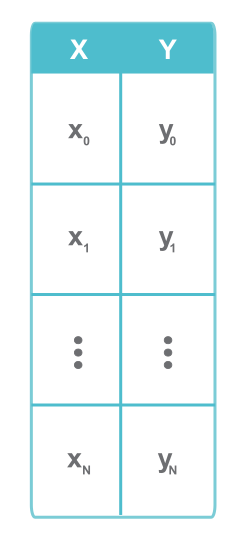
\includegraphics[height=1.35in]{../figs/xy_table}
    \caption{}
    \label{fig:xytable}
  \end{subfigure}
  \begin{subfigure}[t]{0.32\textwidth}
    \centering
    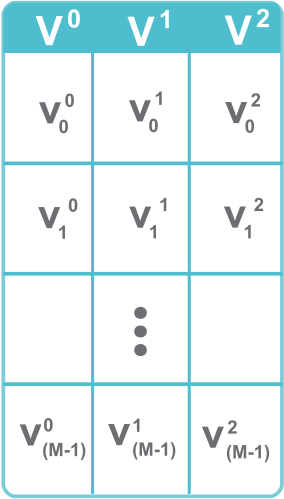
\includegraphics[height=1.35in]{../figs/v_table}
    \caption{}
    \label{fig:vtable}
  \end{subfigure}
  \caption{Examples of an \ugrid{} topology and \cfugrid compliant
    vertex and connectivity arrays. (a) The location of $N$
    vertices in the real plane. (b) A 2D topology with
    $M$ triangles. Each triangle represented as a row in the table
    referencing locations as indices into the vertex array.}
\end{figure}
